% LaTeX file describing how Assignment 10 was done.
% Author: James Cross
% Date: December 10, 2023

\documentclass[12pt]{article}
\usepackage{epsfig}

\begin{document}
\begin{center}
	\large{\textbf{Solving the 2-D Poisson equation using relaxation}}
\end{center}
\raggedright{
The objective of assignment 9 was to solve for the electric potential in a 
grounded 10 cm x 10 cm metal box with two charges inside. This was completed 
numerically by applying a relaxation method to the Poisson equation in a 
program written in FORTRAN 2008.
The Poisson equation (in Gaussian/CGS units) with 
boundary conditions are below,
where $U$ is the electric potential and $q$ is the charge density.
\begin{eqnarray}
	\nabla^2 U(x,y) &= 4\pi q \\
	U(0 \mbox{cm},y) &= 0 \\
	U(10 \mbox{cm},y) &= 0 \\
	U(x,0 \mbox{cm}) &= 0 \\
	U(x,10 \mbox{cm}) &= 0
\end{eqnarray}

The box was discretized into 100 cells on each side with $(i,j)$ representing
the $i$-th cell along the $x$-coordinate and $j$-th cell along the 
$y$- coordinate. The charge distribution was $+4$ in the (75,75) 
cell and $-4$ in the (25,25) cell.
The iterative formula for
the the discretized electric potential at the $i$-th cell along $x$ and the 
$j$-th cell along $y$, is given by the following.
\begin{equation}
	U^{\mbox{new}}_{i,j} = \frac{U^{\mbox{old}}_{i+1,j} 
	+ U^{\mbox{old}}_{i-1,j} + U^{\mbox{old}}_{i,j+1} + U^{\mbox{old}}_{i,j-1}
	- 4 \pi q_{i,j}} {4}
\end{equation}

The resulting potential distribution is shown below.
\begin{figure}[!h]
	\begin{center}	
		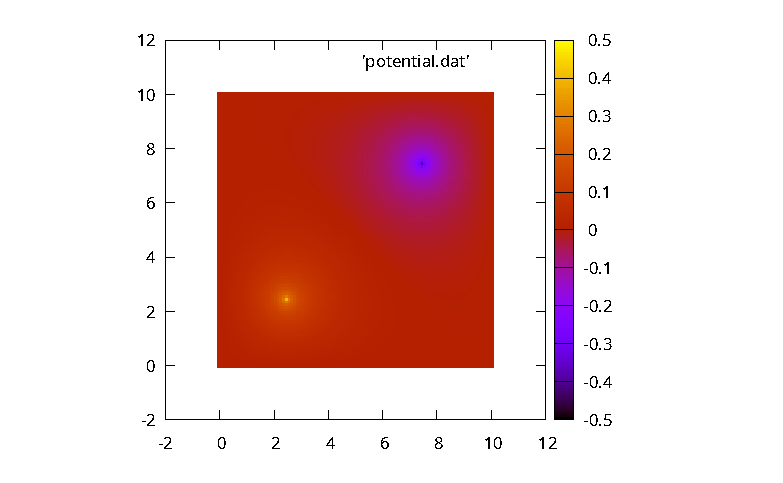
\epsfig{file=james_cross_heatmap.eps,width=0.6\linewidth}
	\end{center}
\end{figure}


}	
\end{document}
